% Class and packages {{{

\documentclass{sig-alternate-2013}

%%%%%%%%%%%%%%%%%%%%%%%%%%%%%%%%%%%%%%%%%%%%%%%%%%%%%%%%%%%%%%%%%%%%%%%%%%%%
% Packages

% \usepackage{algorithm}
%\usepackage{amsfonts}
\usepackage{amsmath}
\usepackage{amssymb}
\usepackage{caption}
\usepackage{color}
\usepackage{comment}
\usepackage{epsfig}
\usepackage{graphicx}
%\usepackage{subfigure}
\usepackage[labelformat=simple]{subcaption}
\usepackage{tabularx}
%\usepackage[hyphens]{url}
\usepackage{hyperref}
\usepackage{wrapfig}
\usepackage[usenames,dvipsnames]{xcolor}
\usepackage{xspace}
\usepackage{multirow}
\usepackage{hyperref}
\usepackage{textcomp}



\usepackage{tikz}
\usepackage{cleveref}
\usepackage{algorithm}
\newcommand*\circled[1]{\tikz[baseline=(char.base)]{
            \node[shape=circle,draw,inner sep=0.5pt] (char) {#1};}}
\newenvironment{widelist}{\begin{list}{$\bullet$}{\setlength{\leftmargin}{.70cm}\setlength{\itemsep}{.00cm} }}{\end{list}}

% Subfigure "Figure 1(a)" style formatting
\renewcommand\thesubfigure{(\alph{subfigure})}

%%%%%%%%%%%%%%%%%%%%%%%%%%%%%%%%%%%%%%%%%%%%%%%%%%%%%%%%%%%%%%%%%%%%%%%%%%%%
% Per-author comment commands
% NOTE: To generate output without comments, build with 'make finalized'.
% This generates a new output file with the suffix '-final.pdf'.

\newcommand{\etal}{et~al.\xspace}

\ifdefined\isFinalized

\newcommand{\todo}[1]{}
\newcommand{\wontfix}[1]{}
\newcommand{\done}[1]{}
\usepackage{ulem}
\normalem
\newcommand{\minor}[2]{{\color{Orange}{\sout{#1}}\color{Blue}{#2}}}
\newcommand{\frank}[1]{{\color{Green}{#1}}}

\newcommand{\addcamera}[1]{#1}
\newcommand{\subcamera}[1]{}

\else

%\newcommand{\todo}[1]{ {\color{Red}{TODO: \emph{#1}} } }
\newcommand{\todo}[1]{}
\newcommand{\wontfix}[1]{}
\newcommand{\done}[1]{}

\usepackage{ulem}
\normalem
\newcommand{\addcamera}[1]{{\color{Blue}{#1}}}
\newcommand{\subcamera}[1]{{\color{Red}{\sout{#1}}}}

\fi

\usepackage{balance}
% }}}
%%%%%%%%%%%%%%%%%%%%%%%%%%%%%%%%%%%%%%%%%%%%%%%%%%%%%%%%%%%%%%%%%%%%%%%%%%%%
% Cleveref configuration {{{

\crefname{figure}{Figure}{Figures}
\crefname{equation}{Equation}{Equations}
\crefname{table}{Table}{Tables}
\crefname{section}{Section}{Sections}
\crefname{subfigure}{Figure}{Figure}

% }}}
%%%%%%%%%%%%%%%%%%%%%%%%%%%%%%%%%%%%%%%%%%%%%%%%%%%%%%%%%%%%%%%%%%%%%%%%%%%%
% Title and authors % {{{


\title{Identifying Synthetic Lethal Interactions in Genes \\ Using Node2Vec and Random Forest}

\author{
 {\setlength{\tabcolsep}{0.48em}
 \begin{tabular}{@{}cccc@{}}
 Cameron Simmons & Aravind Koneru & Hunter Klamut & Namrita Perincherry  \\
 \affaddr{University of Maryland} & \affaddr{University of Maryland} & \affaddr{University of Maryland}& \affaddr{University of Maryland} \\
 \end{tabular}
 }
}

% }}}
%%%%%%%%%%%%%%%%%%%%%%%%%%%%%%%%%%%%%%%%%%%%%%%%%%%%%%%%%%%%%%%%%%%%%%%%%%%%
% Document

\usepackage[override]{cmtt} % make tt font tighter / less ugly


\clubpenalty=10000 
\widowpenalty = 10000 

\hyphenation{de-a-non-y-mi-za-tion}
\hyphenation{none-the-less}
\begin{document}

\urlstyle{tt}

\maketitle

\begin{abstract}
\label{abstract}

Recent advancements in the machine learning field has helped predictions on features of network become more effective. For example, programs from such as Node2Vec have been able to learn continuous feature representations for nodes in networks and learn how to map nodes to a feature dependent dimensional space. As such, Node2Vec has opened the door to much potential research that was not previously easily delved into. In this paper, we investigate the application of Node2Vec to genetic interactions, specifically trying to predict synthetic lethality among interactions. Distinguishing between synthetic lethal and non-synthetic interactions is helpful to the cancer research field, as synthetic lethal interactions can used as a mechanism to target tumor-specific mutations, helping in the development of anticancer therapeutics. The collection of genetic interactions in a species is a network, and therefore, we can use Node2Vec to assist with the learning about the gene interaction network features, such as the type of interaction (synthetic lethal or non-synthetic lethal) between two genes. By using Node2Vec and different machine learning classification models, we demonstrate the proof on concept that by starting with only the genetic interaction network (without the knowledge of each type of interaction), we can make fairly accurate predictions on weather an interaction is synthetic lethal or non-synthetic lethal. Additionally, we explore the idea of merging species by overlapping different species network and connecting them with homologous interactions, seeing if we can get better, more accurate, predictions on genetic interactions.


\end{abstract}


\section{Introduction}
\label{sec:intro}
Genetic interactions are measurements of relationships between genes. For this project, we will be looking to predict synthetic lethal gene interactions (SL) and non-synthetic lethal gene interactions (non-SL). A synthetic lethal interaction occurs between two genes when the perturbation of either gene alone is viable but the perturbation of both genes simultaneously results in the loss of viability (Nigel, 2017). This means that two genes share a SL relationship if a combination of deficiencies in the expression of two or more genes leads to cell death, whereas a deficiency in only one of these genes does not. Otherwise, an interaction between two genes is considered to be Non-SL.

Predicting SL interactions is important because SLs are a mechanism we can use to target cancerous cells. Synthetic lethal genetic interactions with tumor-specific mutations may be exploited to develop anticancer therapeutics. One problem, however, is that predicting SLs can be hard to measure in humans. But, for simplicity, SLs can be measured in model organisms like yeast. In this paper, we look at two model species of yeast, Schizosaccharomyces pombe (Sp) and Saccharomyces cerevisiae (Sc). For both species we are start with a network of genetic interactions and a category for each interaction, SL or non-SL. The ultimate goal is to predict genetic interactions among species accurately. 

After predicting SL and non-SL among each different species, we also ask what would happen if we merged networks from different species. Then using the merged network, would we get better predictions of genetic interactions? The idea behind merging species networks is to use genes that are conserved across species. These genes are called homologs, and they serve similar functions in a pair of species. These genes can be seen as isomorphic to each other. As such, the merging of species is done by overlapping each separate network and connecting cross-species edges with homologous interactions. 

In order to help predict the category for interactions in each species network and the merged network, we used Node2vec to assist with machine learning. Given a network, Node2Vec is able to return a file with vector embedding for each node. 

Through machine learning on individual species networks, we aims to get a proof of concept for graph-vector embedding with genetic interaction networks. Can we make accurate predictions in the synthetic lethality of genes given only a species’ network? Then for the idea of merged species networks, we plan to determine if merging networks of two different species allows for better predictions of gene interactions. In essence, for cross-species networks, we looked at if merging the genetic makeup of two different species would allow us to better understand the gene interaction within the different species. For both the individual species and the cross-species networks, we ran the Node2Vec graph-vector embedding through various different machine learning models, seeing how each model deals with the embedment data, and we  determine which kind of models are best for making prediction on genetic interactions.   Our end goal was to find proof of concept for using graph-vector embedments to help assist with genetic interaction predictions and to make a baseline for merging networks of different species, hopefully to give some insight for future work in this domain.

A significant hurdle in our research was the initial lack of domain knowledge in biology and gene interactions. Throughout the process, we have been having to learning about genetic interactions. Max Leiserson from the University of Maryland - College Park Department of Computer Science, as well as Jason Fan, one of his PhD students, have been working on related areas. Therefore, throughout the semester, we have been collaborating with Jason, and he has been giving us insights on genetic interactions, how to best utilize various machine learning tools, how to merge networks, and ways to get better prediction for interactions. Also, through Jason’s help, we have gained insights to how machine learning on graph representation of genetic interactions can help suggest candidate treatments for cancer. The novel aspect of our approach to identifying SL gene interactions is our use of Node2Vec, a tool released in 2016 to learn patterns in graphs.

Machine learning on graphs, synthetic lethality related to cancer research, and cross-species merging are each not new topics on their own. As such, there are many related works that individually discuss each topic and build up to being able to effectively assist and act as prerequisites for our research. Collectively, the related topics were able to help pose our own questions for new ways of searching for candidate treatments for cancer. Therefore in section 2, we will discuss related works who were necessary prerequisites to completing our projects, as well as a detailed motivation for our own project. In section 3, we will review our methods for obtaining our results, and in section 4, we present our results. Ultimately, in sections 5, we suggest future work based off the groundwork of our research and the results we were able to achieve. 

%\newpage
\section{Background and Related Work} % {{{
\label{sec:background}

\subsection{Machine Learning on Graphs and Node2Vec} % {{{
\label{sec:node2vec}

Node2Vec is one of the prominent applications used to support the findings in this study. In the field of machine learning, often a set of features is known prior to solving a problem; however, Node2Vec's purpose is to provide an algorithmic framework for learning continuous feature representations for neural network nodes when the features are not so obvious. Node2Vec aims to add flexibility in exploring neighborhoods of nodes, or nodes that are grouped closely together. The program itself aids in multi-label classification (attaching multiple valid labels to an input) and link prediction (estimating which nodes are likely to have edges connecting them).

In terms of genomics, multi-label classification comes into play when attaching likelihood of a gene being synthetic lethal or not. Likewise, link prediction comes into play to gauge whether any two genes have interactions with one another. Thus, one can see how useful this algorithm to learn features is with respect to studying cancerous patients; given data about those afflicted with cancer, Node2Vec learns which features of the data given are the most likely to be related to the cancer as well as which features are intertwined.

Node2Vec's algorithm is semi-supervised. Humans at first decide which features to throw into the algorithm, but Node2Vec ultimately weights these features and determines which are worthwhile. Its goal was to be more flexible and scalable than the previous feature learning algorithms that existed. To do this, Node2Vec incorporated parameters the programmer can tune upon execution, particularly the random walk size and the search bias. The walk size determines the extent to which the algorithm explores nodes from a given source, and the search bias is the likelihood with which Node2Vec returns to nodes it has already explored. Tweaking these parameters can give vastly different depictions of the features learned by the network. As such, they are useful for exploring any data presented from a variety of angles.

Fine-tuning the neural network occurs in a sequence of three steps: preprocessing and computing of transition probabilities, random walk simulations, and finally optimization using stochastic gradient descent. The preprocessing involves a variety of calculations which determine the likelihoods to which given nodes are related prior to any walk. Then the random walk simulations effectively traverse the network's pathways in an effort to explore relatedness of nodes in a framework consistent with the walk size and search bias parameters. Finally, stochastic gradient descent iteratively calculates the partial derivative of the cost function with respect to the input vectors and adjusts the weights in the network accordingly (the learning aspect).

Node2Vec, because of the freedom to tune the walk size and search bias, can depict novel relationships between nodes. For example, having a large walk size with a low search bias (low likelihood to return to previous nodes) will likelier depict a network in which nodes are connected for long distances but are not grouped as much in neighborhoods. Decreasing the walk size and increasing the search bias depicts a scenario where nodes are not connected by edges for long pathways but neighborhoods of nodes are emphasized. Clearly, this flexibility is useful as it pertains to machine learning in cancer research; researchers can apply hypotheses to the algorithm in novel ways and based on what they predict, fine-tuning of the parameters could give new insights.

Ultimately, Node2Vec is useful mainly for its scalability and flexibility especially with respect to feature learning in bioinformatics. Node2Vec was employed in order to analyze the extent to which genetic interactions occurred in the two yeast species. Because of the scalability, there were no issues analyzing the amount of data present; because of the flexibility, it was possible to analyze link prediction for genetic interactions within the two species as well as the homologs of interactions between the two species.



\subsection{Genetic Interactions In Yeast and synthetic lethality regarding cancer} % {{{
\label{sec:genetic_interactions}
Genetic interactions is a measure of the effect of a modification in one gene on another gene. For our research, we are particularly interested in synthetic lethal interactions. Synthetic lethality involves multiple genes, where the loss of either gene alone has very little impact on the cell, but the loss of all the genes in the interaction leads to a massive decrease in fitness or even cell death (Madhukar, Elemento, \& Pandev, 2015). SL interactions are difficult to measure in humans, thus our interest in predicting these interactions. These interactions have very important significance in the world of biology and medicine, for predicting them can provide therapeutically exploitable weaknesses in tumors. All genetic interactions can be very broadly classified as positive or negative, explaining whether the interaction increased or decreased the gene’s fitness (Jasnos and Korona, 2007). The interactions are crucial in describing functional relationships among genes and their corresponding proteins, as well as explaining complex biological processes and diseases. Synthetic lethality is one of the most significant and researched gene interaction, because it is the extreme case of a negative interaction.

Synthetic lethality can be used to selectively target cancer cells. Predicting SLs have been successful in pharmacological PARP inhibition in BRCA-mutated tumors (Weil and Chen, 2011). However, predicting these synthetic lethal interactions can go far beyond that. Many somatic mutations in cancer genes cannot be targeted directly, however, some may be actionable through the identified synthetic lethal interactions (Emerling et al., 2013). Standard chemotherapy approaches for cancer were previously discovered on the basis of their ability to kill cells which divide rapidly. The toxicity to these dividing cells are a cause for the side effects of chemotherapy, such as hair loss, nausea, and immunosuppression (Chan and Giaccia, 2013). In hopes of reducing these side effects, cancer research in the past has been largely focused on identifying traits which are tumor-specific and may be exploited for selective targeting. 

The DNA mutation rate is very low in normal cells, but there are many somatic mutations in cancer cells. A drug that targets the synthetic lethal partner gene of a cancer-specific mutated gene will kill the cancer cells, whilst sparing the normal cells. Originally, SL was discovered in genetic experiments of yeast and fruit fly. It was proposed by Hartwell et al as a new framework for anticancer therapies in 1997, and has been intensely researched since. More recently, an SL-based drug, specifically the inhibitor of poly ADP-ribose polymerases (PARPs), which has synthetic lethal interactions with the BRCA1 and BRCA2, two well-known genes whose mutations lead to breast cancer, has achieved clinical success for breast cancer therapy. The main approach to discovering SL is screening using RNA interference. However, SL screening has limitations due to high cost, false-positives, lack of mechanistic interpretation, and inconsistency among cell lines (Conde-Pueyo \& Munteanu, 2009). Thus, very few SL pairs have been discovered in human cancer. Yeast is an extremely popular model organism for human research due to the abundant data of genetic interactions, including synthetic lethal. 

Yeast is one of the simplest eukaryotic organisms. It is an extremely important organism for biological research because many essential cellular processes are the same in yeast and humans. By studying yeast, researchers gain more of an understanding on basic molecular processes in humans. However, even for yeast, only a small portion of gene pairs have been covered using synthetic lethal screening. For this reason, relying on computational methods is extremely important for large-scale discovery of synthetic lethal interactions. In the past decade, several machine learning method have been proposed and tested on the benchmark datasets of yeast, which revealing that computational methods do have great potential in analyzing and predicting SL (Qi, Suhail, Lin, Boeke, \& Bader, 2008). Qi et al applied diffusion kernels defined on the network of yeast SL interactions in a support vector machine classifier for the prediction of novel genetic interactions and protein co-complex membership. Palagudu et al extracted many features from protein-protein interaction entwords, which were used in an SVM to predict new synthetic lethal interactions. Both of these methods tend to focus on a particular type of features and use a single machine learning method. However, as SL interactions are highly complex, they are likely to be caused by different mechanisms. Thus, our goal was to provide a more integrative analysis of multiple features.


\subsection{Intelligent Merging of Species} % {{{
Organisms are constantly interacting with other species through physical contact, leading to changes on a molecular level. The goal of intelligently merging species is to combine multiple heterogeneous networks with different connectivity patterns, to achieve more accurate inferences. However, there are many challenges when it comes to transferring knowledge between species. Mainly, different species have different genetic architectures. However, because of the availability of complete genomic sequence of humans and other species, the opportunity for understanding gene functions is tremendous. Gene function can be inferred in multiple ways, including DNA microarray expression data. Microarrays now allow biologists to formulate models of gene expression on a larger scale than anything that has been seen several years ago. 

Initially, analysis of this data focused on clustering algorithms and self-organizing maps, which attempt to automatically locate clusters of genes with similar expression patterns, thus they may share similarity in function. However, recently, methods have been created to apply a collection of learning techniques to a set of microarray expression data from yeast using kernel methods. Merging species will lead to improved performance, due to the kernel’s ability to incorporate prior knowledge about the heterogeneity of the data. Prior knowledge of heterogeneity should be exploited when choosing subsets of input features for use in classification (Pavlidis, Weston, Cai, Grundy, 2001). Feature selection is extremely important to intelligently merging species. 

There have been computational approaches to transfer knowledge between species, which have mainly relied on measures of heredity, ie. genetic homology (Fan, Cannistra, Fried, Lim, Shaffner, Crovella, Hescott, \& Leiserson, 2018). However, only a small subset of genes do have homologs, which limits the amount of transferable knowledge. Genes also repurpose and change functions, further complicating this transfer of knowledge. 

Fan et al has taken a different approach to transferring knowledge across species by using explicit measures of functional similarity of proteins between species to expand on the notion of homology. Using a kernel-based method, Homology Assessment across Networks using Diffusion and Landmarks, has allowed for the ability to integrate sequences and network structures to create embedding where proteins from different species are included in the same vector space. HANDL-embedding can co-locate gene pairs with synthetic lethal interactions in HANDL-space both within and across species. HANDL provides homology scores for gene pairs in different species with are associated with pairwise gene function. Fan et al used HANDL to identify synthetic lethal interactions between S. cerevisiae (S.c.) and S. pombe (S.p.), which are two different species of yeast. HANDL allows for the training of classifiers for multiple species, rather than usual SL prediction methods which do not account for multiple species. 

Mashup is a framework designed for scalable and robust network integration where diffusion in each network is first analyzed to characterize the topological context of nodes. Then, the topological patterns in each individual network are shown using low-dimensional vectors, one per gene or protein. Using these vectors, one can use machine learning to derive functional insights about genes, specifically, genetic interaction (Cho, Berger \& Peng, 2016). 

Although different approaches have been taken to intelligently merge species, we used the data from HANDL on S. cerevisiae and S. pombe to determine a better way of predicting synthetic lethal interactions. Intelligently merging species has many different uses, however, for the purpose of this research topic, we focused on intelligently merging species to predict synthetic lethal interactions between genes. 


%\newpage
\section{Methods}
\label{sec:methods}
For our research, we used the following initial datasets: 

\href{https://obj.umiacs.umd.edu/lrgr/ppi-gi-data/gi/collins/sc/collins-sc-emap-gis-std.tsv
}{\textit{Dataset Sc}}

\href{https://obj.umiacs.umd.edu/lrgr/ppi-gi-data/gi/roguev/sp/roguev-sp-emap-gis-std.tsv
}{\textit{Dataset Sp}}


The file, collins-sc-emap-gis-std-tsv, contains a representation of the gene interactions networks in Sc yeast, and roguev-sp-emap-gis-std.tsv contains a representation of the gene interactions networks in Sp yeast. Each data file contains a list of edges in the respective network, geneA interacting with geneB, and a category for each interaction, SL, Non-SL, or Inconclusive. The data set also provides an S-score for each interaction, but for our project, we are not concerned with the S-score.

The first step for this data is to generate a runnable edgelist file that can be used as input for the Node2Vec program. Since Node2Vec only allows for integers in the runnable edgelist file, we started by assigning unique integer id values to each gene in both files. We were then able to build the runnable file. Note that the runnable edgelist file does not contain any edge-weights, so the Node2Vec will not take into account whether a given gene interaction is SL or Non-SL. Node2Vec only knows that an interaction merely exists between two genes. We used the default values for Node2Vec, that is 128 dimensions, 80 length of walk per source, 10 walks per source, 10 context size of walks per source, 1 epoches in SDG, undirected, and unweighted. Each parameter for Node2Vec is described in their paper (Grover, 2016). With the embedded file from Node2Vec’s output, we have each gene’s id assigned to a 128 dimensional vector. From there, we were able to reassign the genes to their respective vector using the id data. We were are also able to construct a file of the following format for each gene interaction: geneA, Adim1-Adim128, geneB, Bdim1-Bdim128, score, category. This shows that gene A interacts with gene B, and provides the vector for both gene A and gene B, as well as their category (SL, Non-SL, or Inconclusive). From there, in order combine both interacting genes into a single vector that describes their relationship, we took the Hadamard product of each gene interaction, having a file with the following format: geneA, geneB, HadamardDim1-HadamardDim128, score, category. Note that we made this kind of file format for both Sc and Sp, two separate files. 

In order to prepare for machine learning, we made the note that there are many more Non-SL interactions than SL interactions for both sets of data. In the Sp yeast, there were 5,516 SL interactions and 99,079 Non-SL interactions. In Sc yeast, there 7,239 SL interactions and 125,604 Non-SL interactions. For the sake of machine learning classification, we wanted to keep the number of data points for each type even, so for each file, we took all of the SL interactions and a random sample of the same of Non-SL as SL . This means for the Sp yeast, we had all 5,616 SL interactions and 5,616 randomly sampled Non-SL interactions. Then in the Sc yeast, we have all 7,239 SL and a random sample of 7,239 Non-SL interactions. Note that all inconclusive interactions were excluded, as we can’t train nor cross-validate with inconclusive data. 

At this point, we were fit to continue onto running machine learning model on both species in order to predict whether an interaction is SL or Non-SL. We ran the data through six different classifiers: logistic regression, naive bayes, decision tree, support vector clustering, random forest, and k-nearest neighbor. We only makes predictions based off the 128 dimensions of the Hadamard product, excluding score. 70\% of the data was used for training data, and the remaining 30% of data was testing data.

After making predictions on individual species, we shifted our focus to cross-species networks. To merge the species, Sp and Sc, we acquired the following homolog dataset:

https://obj.umiacs.umd.edu/lrgr/ppi-gi-data/homologs/sc-sp/sc-sp-homologs.txt

This file is a list of all of the homologs shared by Sp and Sc yeast. For merging, we overlapped both species’ networks and connected them via the homologs. From there, the same process occurred for the merged network as we did for the individual species network: we assigned ids to the genes, made a runnable file for Node2Vec, took the Hadamard product, took all of the SL interactions, randomly sampled the Non-SL interactions, and ran the classifier models on the networks. We had three kinds of merged files: two were Sp merged and Sc merged, where we merged the networks for Node2Vec and then separteted them again for machine learning classification, and other one is ScSp merged, merging during both Node2Vec and the machine learning classification. 

In the following sections we discuss the machine learning classification results for all 5 kinds of datasets: Sp, Sc, Sp merged, Sc merged, and ScSp merged. 

\newcommand*{\figuretitle}[1]{%
    {\centering%   <--------  will only affect the title because of the grouping (by the
    \textbf{#1}%              braces before \centering and behind \medskip). If you remove
    \par\medskip}%            these braces the whole body of a {figure} env will be centered.
}

\section{Results}
\label{sec:validation}

Upon running our trained models on the dataset, we identified some classifiers that were doing
better than others in terms of successfully classifying genetic interactions as SL. This table
presents the top classifiers for each dataset that we tested. In every case, Random Forest was the
highest performing classifier. In general, it seems that using a random forest will correctly
estimate about 70\% of the SL gene interactions. 

An initial concern was that our model was over-fitting the tree due to the 100\%
classification accuracy on the training data. To check that we weren't over-fitting, we re-trained
the models with a smaller forest size to see if the training data accuracy would change. Our
results are presented in table \emph{X}. Despite changing our forest size, the model maintained an
accuracy of 100\% on the training data but with consistent drops in test data classification. From
these results, we came to the conclusion that using a tree size of 128 or 256 would be ideal since
it would maximize test data classification. Further research is necessary to determine if the
relationship between forest size and test accuracy is parabolic in nature or is upper bounded. 

\begin{figure}[t!]
\centering
%
\figuretitle{Classifer Results}
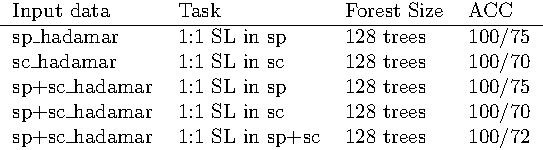
\includegraphics[width=.48\textwidth]{figs/best-class}
%
\end{figure}

% }}}

% Accuracy as a function of path length plots {{{

\begin{figure}[t!]
\centering
%
\figuretitle{Changing Forest Size}
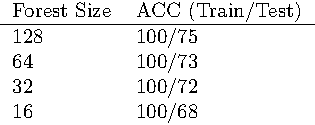
\includegraphics[width=.38\textwidth]{figs/forest-size}
%
\end{figure}

Given that the initial results were very promising, we took a closer look at the model for the Sp to
determine if the model could be reliable over a larger dataset. We ran a stratified 5 fold cross
validation instead of a normal 5-fold cross validation since we are dealing with classification and
want about an equal number of each type in each split. After running the model through validation,
we found that the model's accuracy was consistent around 75\% which is the same result we initially
received. This means that the model could be applied to other datasets and would be minimally
affected by bias. We would test this theory, but the lack of relevant data make testing across
two different datasets difficult. Furthermore, we were surprised to find that that even random
forests with smaller forest sizes yielded fairly consistent results when put through the same
stratified 5 fold cross validation. 

\begin{figure}[t!]
\centering
%
\figuretitle{Stratified 5 Fold for Size=128}
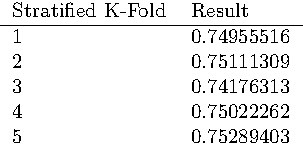
\includegraphics[width=.38\textwidth]{figs/strat-128-dim}
%
\end{figure}

% }}}

% Accuracy as a function of path length plots {{{

\begin{figure}[t!]
\centering
%
\figuretitle{Stratified 5 Fold}
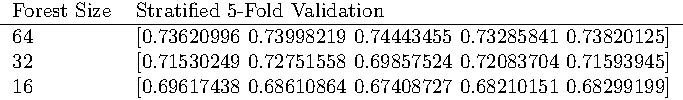
\includegraphics[width=.48\textwidth]{figs/strat}
%
\end{figure}

The PR curve of our model isn't ideal, but it shows that our model has promise and can be improved.
The baseline is 50\% and it appears that for about 50\% recall we can have 75\% precision which is
very reasonable. This could be further improved by trimming the feature set or playing around
with how different input vectors would change results. We firmly believe that our research shows that there is more work to be done studying how graph analysis tools like node2vec can be used to study genetic interactions. The area under our ROC curve is .75, which is a strong indicator that the random forest does a good job of differentiating the different classes. Something else we noticed was that the identification rate for both SL and non-SL were about the same which suggests that there might be value in trying to indentify non-SL interactions and assume interactions not classified are SL. Once again, this is an opportunity for further research. 

\begin{figure}[t!]
\centering
%
\figuretitle{ROC Curve}
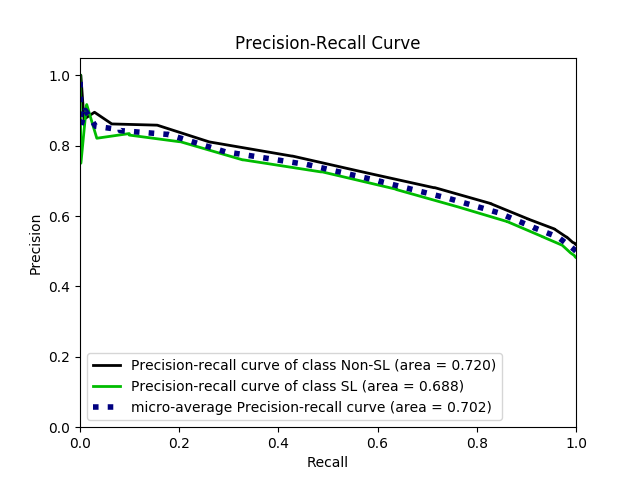
\includegraphics[width=.48\textwidth]{figs/pr-curve}
%
\end{figure}

% }}}

% Accuracy as a function of path length plots {{{

\begin{figure}[t!]
\centering
%
\figuretitle{PR Curve}
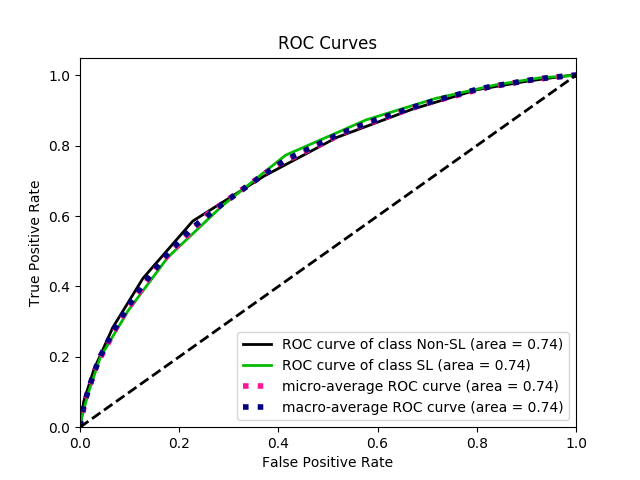
\includegraphics[width=.48\textwidth]{figs/testplot}
%
\end{figure}


%% \section{Related Work}
% \label{sec:related}

% Ting builds upon and attempts to complement three perpendicular fields of related work: (1) denanonymization of Tor circuits, (2) improvement of Tor path selection algorithms, and (3) large-scale network measurement. 

% \if 0
% \subsection{Deanonymization} %{{{

% \begin{itemize}
% \item Practical Congestion Attack on Tor: Adversary controls an exit node, injects javascript into each request forcing client to ping exit node at fixed rate. Adversary then floods possible entry nodes one-by-one until delay is observed in ping time. \cite{practical-congestion}
% \item How Much Anonymity Does Network Latency Leak?: (1) Two colluding web serves determine if pair of connections came from same Tor user or two different users by comparing distrubtions of RTTs of entire circuit. (2) Suggest ability to triangulate a client from a series of Murdoch-Danezis attacks with the help of Vivaldi or King. \cite{latency-leak}
% \item Low Cost Traffic Analysis of Tor: the first significant paper on deanonymizing Tor. Introduces the Murdoch-Danezis attack cited / built-upon by many later attacks. Attack involves using a malicious web server to introduce a distinct traffic pattern in a stream then probing nodes until that same pattern is found \cite{low-cost-traffic-analysis}. \cite{practical-congestion} proves that it no longer works given the current size of the Tor network because there's too much noise.
% \item User's Get Routed: Traffic Correlation on Tor by Realistic Adversaries: Current method takes up to three months for a typical Tor relay, good candidate for being sped up by ting! \cite{get-routed}
% \item Syping in the Dark: TCP and Tor Traffic Analysis: assume adversary can eavsdrop on clients but not on network, goal is to determine if any clients are trying to access restricted site S, attack by inducing TCP congestion between exit relay and S and observing which clients are affected by it. \cite{spying}
% \item TorScan: Tracing Long-Lived Connections and Differential Scanning Attacks: given a relay X, they claim to be able to exploit the Tor protocol messages to determine all other relays that X is directly connected ot in a circuit. Given this, if they control an exit node, then they know the second node, and can scan the second to find the first. Downside is this is only practical for long-lived connections (ssh, large files, IM).\cite{torscan}
% \item Traffic Analysis Against Low-Latency Anonymity Networks Using Available Bandwidth Estimation: same kind of attack as others but induce and monitor bandwidth fluctuations as opposed to latency. \cite{bandwidth-analysis}
% \end{itemize}

% % }}}
% \fi

% \if 0
% \subsection{Path Selection} % {{{

% \begin{itemize}
% \item \todo{Still need to find some of these...}
% \end{itemize}

% % }}}
% \fi

% \subsection{Measurement} % {{{

% \begin{itemize}
% \item IDMaps: requires large amount of additional infastructure which isnt very practical in terms of cost, deployment, and speed. Has been outdone by many successors such as King. \todo{is this appropriate, since King mentioned it as a related work, and already proved it was better than ID Maps?} \cite{idmaps}
% \item King: lightweight tool for measuring the latency between two arbitrarily-selected end hosts. Finds a DNS resolver near each host (one must support recursive requests), then sends a DNS query which traverses the path between the two servers, and uses subtraction to find the latency. Makes the assumption that end hosts are geographically near their local DNS server. \cite{king}
% \item Estimating Hop Distance Between Arbitrary End-Host Pairs: requires deployment of additional infastructure, and still only computes estimates, rather than traversing the entire path. \cite{estimating-hop-distance}
% \item Predicting Internet Network Distance with Coordinates-Based Approaches: uses algorithms based on geometric model of the Internet to predict latencies. May produce accurate results in general, but is not related to the current state of the path between two nodes, and thus would not be useful for looking at latencies changing over time or in response to events.  \cite{predicting-network-distance}
% \item Pathchar: similar technique as traceroute, but gathers more statistics. Uses same basic idea of subtracting components from a sum which contains the desired measurements. \cite{pathchar}
% \item Vivaldi: algorithm for computing syntehtic coordinates for intnernet hosts -- no required infastructure, only needs to contact a few other hosts to gain enough information about itself, scales well, median relative error of 11\% for embedding 1740 Internet hosts within a 2d Euclidiean model \cite{vivaldi}
% \item Treeple: Latency estimation between peers in a distributed system based solely on their position. Unique qualities: (1) provably more secure than previous methods, (2) positions based on actual network topology rather than Euclidiean coordinates, (3) highly stable, do not require maintainence very often. Median relative error is 26\% for dataset of 200,000 measurements (Vivaldi was 25\%) \todo{could we compare to this same dataset?}\cite{treeple}
% \item Sequoia (treeness of Internet latency): system for embedding latency and bandwidth into trees, can be used for server selection,.. \cite{sequoia}
% \item Netvigator: network proimity and latency estimation tool that uses information obtained from probing small number of landmark nodes and intermediate routers to identify closest nodes \cite{netvigator}
% \item Global Network Positioning: models the Internet as a geometric space and computes geometric coordinates to characterize positions of hosts in the Internet, used to accurately predict network distances \cite{gnp}
% \item NetFlow Latency Estimation: utilizes existing NetFlow architecture, approximates delay samples from other background flows, has median relative error of less than 20\% for flows of size > 100 packets \cite{netflow}
% \item Htrae: \cite{htrae}
% \item iPlane: \cite{iplane}
% \item Tor Metrics? \cite{tor-metrics}
% \end{itemize}


% % }}}

\section{Conclusion}
\label{sec:conclusion}

From our results, we are able to conclude that the idea of predicting SL and Non-SL using graph-vector embedding from programs like Node2Vec is plausible. Predictions can be made given only a network of genetic interactions. We were also able to get a sense of which kind of machine learning classification models work best, such as support vector clustering, random forests, and k-nearest neighbors. However, our best prediction was just over 75\%, with many other prediction model being a fair bit lower. In the future, we aim increase this accuracy.

One idea to increase the accuracy of the models is to further explore the parameters of Node2Vec. For this paper, we merely used the default values for Node2Vec. There may be parameters that can be explored and tweaked  that may lead to a better graph-vector embedding. Additionally, there are other programs such as GraphSAGE, released in 2017, that also may be able to assist in finding relevant features on networks (Hamilton, 2017). Perhaps combining Node2Vec and GraphSAGE results could lead to better predictions. 

Another idea to improve prediction accuracy is to further explore the top-performing machine learning classification models. For all of the models we used, we loosely explored tweaking the model parameters. Perhaps within each model, tweaking certain parameters may lead to better predictions. Additionally we could try to taking the consensus prediction for the top-performing models, and see if using the consensus leads to better predictions.

Finally, our results show that our method of merging for cross-species predictions was not sufficient for improving prediction accuracy, but it also didn’t decrease accuracy. In the future, other merging methods may be explored. One such method that may be further explored is a cross-species merging technique used by Jason Fan, a computer science PhD candidate from the University of Maryland, in his work with HANDL (Homology Assessment across Networks using Diffusion and Landmarks).

By better exploring parameters for both Node2Vec and the machine learning classification models, getting assistance from other programs like GraphSAGE, and finding better methods for cross-species merging, future work may leading to better prediction for SL and Non-SL interactions.


\section*{Acknowledgments}

We would like to thank Max Leiserson from the University of Maryland - College Park Department of
Computer Science for introducing us to the topic of predicting synthetic lethality and how it can be
used for cancer related research. We would also like to thank Jason Fan, Leiserson\textquotesingle s
PhD candidate
student, who has been able to help guide our works by providing insights on Node2Vec and help make prediction and other suggestions on how to carry out our work.  




\balance
\nocite{*} 
\bibliographystyle{abbrv}
\bibliography{main}

\end{document}

